% ----------------------------------------------------------
\chapter{Desenvolvimento da Aplicação}
% ----------------------------------------------------------

Na extensão deste capítulo serão abordadas as técnicas, decisões de projeto e desenvolvimento da aplicação proposta nos objetivos do trabalho, implementando o método descrito no Capítulo 3 como estrutura de codificação de dados e apresentando um \textit{software} capaz de inserir uma mensagem arbitrária dentro de um arquivo binário de código compilado.

\section{Escolha de Linguagem e Definições Gerais do Projeto}

\subsection{Linguagem e Ambiente}

Para todos os desenvolvimentos práticos foi definido o uso da linguagem Python, conhecida por sua simplicidade e clareza de código, o que facilita a compreensão para os pesquisadores e desenvolvedores de diversas áreas, em sua versão 3.10. Além disso, a vasta gama de bibliotecas e módulos disponíveis em Python, como \texttt{struct}, \texttt{pickle}, e \texttt{array}, oferece funcionalidades prontas para o tratamento de dados binários, economizando tempo e esforço no desenvolvimento. A portabilidade do Python também é uma vantagem, já que a linguagem é suportada em diferentes sistemas operacionais, garantindo que os resultados do projeto sejam facilmente reproduzíveis. Por fim, a comunidade Python ativa e os recursos de documentação tornam mais simples a resolução de problemas e o suporte durante o desenvolvimento do projeto.

Até o momento da publicação dessa monografia não existe uma forma obrigatória definida pela linguagem de como estruturar seus projetos, portanto foram seguidas as recomendações dadas no livro \textit{The Hitchhiker's Guide to Python} que são utilizadas em larga escala pela comunidade \cite{reitz2016hitchhiker} em conjunto com o gerenciador de dependências Poetry utilizado para distribuir de forma homogênea a aplicação em diversas máquinas \cite{poetry}.

\subsection{Estrutura de módulos}

A aplicação está organizada em módulos Python com responsabilidades distintas a fim de hermetizar cada funcionalidade em um único local e evitar dependências desnecessárias e facilitar a manutenabilidade de cada módulo. Em seguida estão descritos os módulos com relevância para o entendimento da implementação da técnica proposta no capítulo passado.

\subsubsection{\texttt{arch.riscv}}

Esse módulo contém os arquivos responsáveis por todo tipo de transformação e operação relacionadas com a arquitetura RISC-V, como o decodificador de instruções, codificador de instruções e os próprios formatos de instruções e seus campos. Todas as classes foram desenvolvidas seguindo uma interface definida em um módulo de definição denominado \texttt{arch.common} para facilitar uma implementação futura de outras arquiteturas.

\subsubsection{\texttt{elf}}

Módulo responsável por decodificar arquivos no formato ELF a partir de uma estrutura de dicionários aninhados e enumerações que seguem a especificação técnica da extensão, oferecendo suporte para o \textit{parsing} de segmentos, seções e tabelas de símbolos, além de um sumário do cabeçalho principal do arquivo.

\subsubsection{\texttt{handlers}}

Contém as funções responsáveis por receber os argumentos da execução do programa e executar a lógica de cada operação de alto nível disponível para o usuário. Para cada comando disponível para o usuário, existe um arquivo de \textit{handler} homônimo encarregado de implementar entrada, processamento e saída daquele comando, essa estrutura é sugerida pela biblioteca \texttt{click} e facilita a adição de novos comandos na aplicação.

\subsubsection{\texttt{utils.binary\_manipulation}}

Esse módulo simples contém algumas operações comuns para serem aplicadas em dados binários, como inversão de ordenamento de bytes, complemento de 2 e extensões de sinal. Outros módulos como o \texttt{arch.riscv} e \texttt{elf} se aproveitam dessas funções disponíveis para simplificar suas próprias lógicas internas.

\subsubsection{\texttt{utils.crypto}}

Durante o processo de codificação e decodificação de mensagens embutidas em arquivos binários existe também uma camada de criptografia que é implementada por este módulo, que na prática apenas encapsula funcionalidades da biblioteca \texttt{pycryptodome} de forma mais amigável para um programador, oferecendo operações de alto nível compostas por uma série de operações menores a fim de prover ao usuário uma forma segura e simples de criptografar e descriptografar porções arbitrárias de dados.

\subsection{Estrutura de Execução da Interface}

A aplicação foi organizada de forma a expor suas funcionalidades por meio de uma interface de linha de comando, utilizando a biblioteca \texttt{click} que permite a declaração de comandos a partir anotações de decoradores em funções da linguagem. O comando lê a entrada fornecida pelo usuário verificando se todos os parâmetros obedecem obrigatoriedade e tipos definidos pela interface, levantando exceções legíveis caso algum dado passado falhe na checagem. Em seguida o \textit{handler} inicia o processamento do comando e retorna a saída para o usuário, encerrando o fluxo de uma chamada do programa.

\subsection{Comandos Disponíveis}

\subsubsection{\texttt{encode}}

O comando \texttt{encode} é responsável por receber uma mensagem em texto plano, criptografá-la e inserir-la no arquivo de fonte, gerando ao final o estego-objeto. Para os propósitos deste trabalho foi utilizada criptografia simétrica com o algoritmo AES sendo instanciado em \textit{Output Feedback Mode}, uma modalidade do AES que trabalha de forma serial utilizando o vetor de inicialização para gerar o texto cifrado de forma iterativa, com uma operação \textit{XOR} entre o texto e um bloco cifrado a partir da chave, gerando uma distribuição de probabilidade pseudoaleatória para cada bit da mensagem cifrada final \cite{Dworkin2001}. Todas as chaves são derivadas a partir de uma senha escolhida pelo usuário utilizando PBKDF2, uma função computacional capaz de derivar chaves pseudoaleatórias a partir de uma entrada em texto plano, utilizando como função de \textit{hash} HMAC-SHA512, com $2^{15}$ iterações e um \textit{salt} de 16 bytes \cite{Turan2010}.

Após criptografada a mensagem é concatenada ao \textit{salt}, codificada em \textit{base64}  e inserida conforme definido no Algoritmo \ref{alg:one}, adicionando um caractere de final de mensagem para delimitar o tamanho total do texto inserido e utilizar como critério de parada no processo de decodificação. Nesse passo foi realizada uma otimização de implementação no algoritmo, o parâmetro de entrada \textit{P} é fornecido a partir de uma função do tipo \textit{generator}, que age como um objeto iterável retornando a cada iteração uma instrução do programa. Dessa forma, mesmo que seja utilizado um arquivo de tamanho elevado as instruções são trazidas para memória apenas quando serão utilizadas, resultando em diminuição drástica do uso de recursos para execuções em grandes arquivos.

O arquivo modificado é salvo em caminho alternativo ao original, a partir de uma cópia do original, alterando apenas as instruções codificadas no programa o que diminui o número de operações em disco realizadas pela implementação, dessa forma o usuário mantém o objeto de cobertura intacto e recebe um estego objeto recém criado. Caso a mensagem exceda a capacidade de codificação do arquivo informado é levantada uma exceção que alerta o usuário sobre o ocorrido e o arquivo não é alterado em nenhum aspecto. O funcionamento completo do comando de codificação está ilustrado na Figura \ref{fig:encode}.

\begin{figure}[!htb]
     \centering
     \caption{Esquemático do funcionamento do processo de codificação.}
     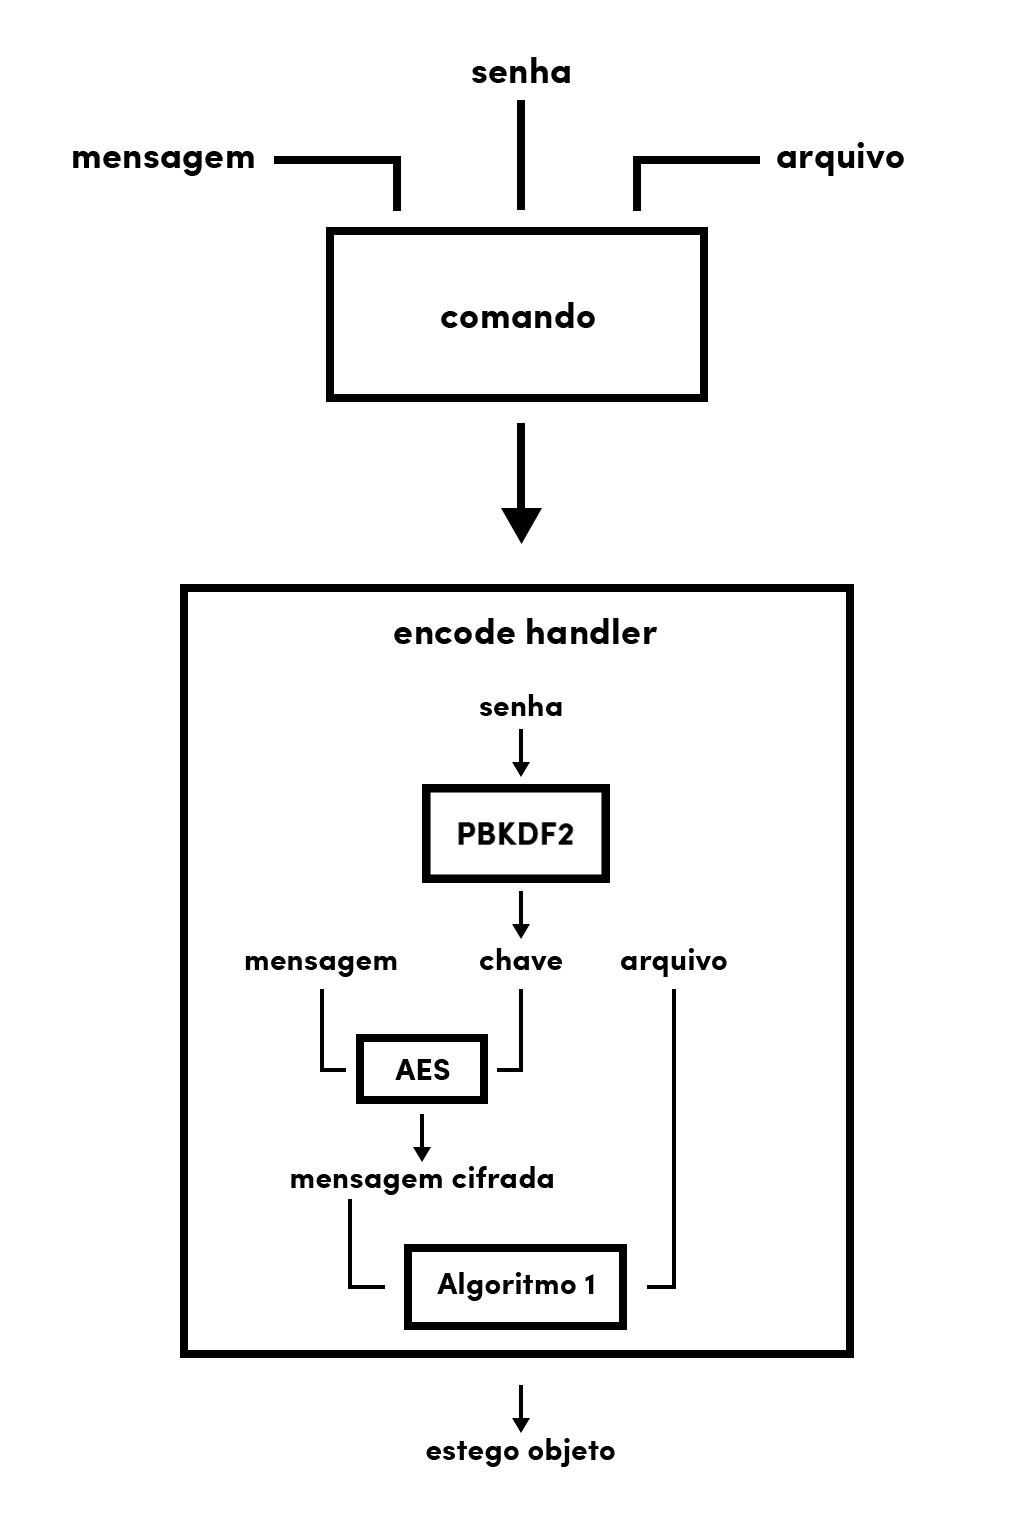
\includegraphics[width=10cm]{images/TCC4.png}
     \legend{Autor: Imagem produzida pelo Autor}
     \label{fig:encode}
\end{figure}

\subsubsection{\texttt{decode}}

O processo de decodificação é realizado de forma inversa a codificação, recebendo um arquivo binário que se presume ser um estego objeto criado com a mesma técnica e uma senha para descriptografar a mensagem. Inicialmente buscamos toda a mensagem criptografada contida no arquivo, utilizando o Algoritmo \ref{alg:two} como base até encontrar um caractere de parada, caso nenhum caractere de parada seja encontrado a aplicação levanta uma exceção alertando o usuário de que o arquivo não contém dados relevantes inseridos em si. Ao encontrar uma mensagem geramos uma chave a partir da senha utilizando PBKDF2 e o \textit{salt} contido no início da mensagem, ao ponto em que podemos descriptografar a mensagem utilizando o AES com a chave derivada e retornar a mensagem em texto plano para o usuário. O funcionamento completo do comando de codificação está ilustrado na Figura \ref{fig:decode}.

\begin{figure}[!tb]
     \centering
     \caption{Esquemático do funcionamento do processo de decodificação.}
     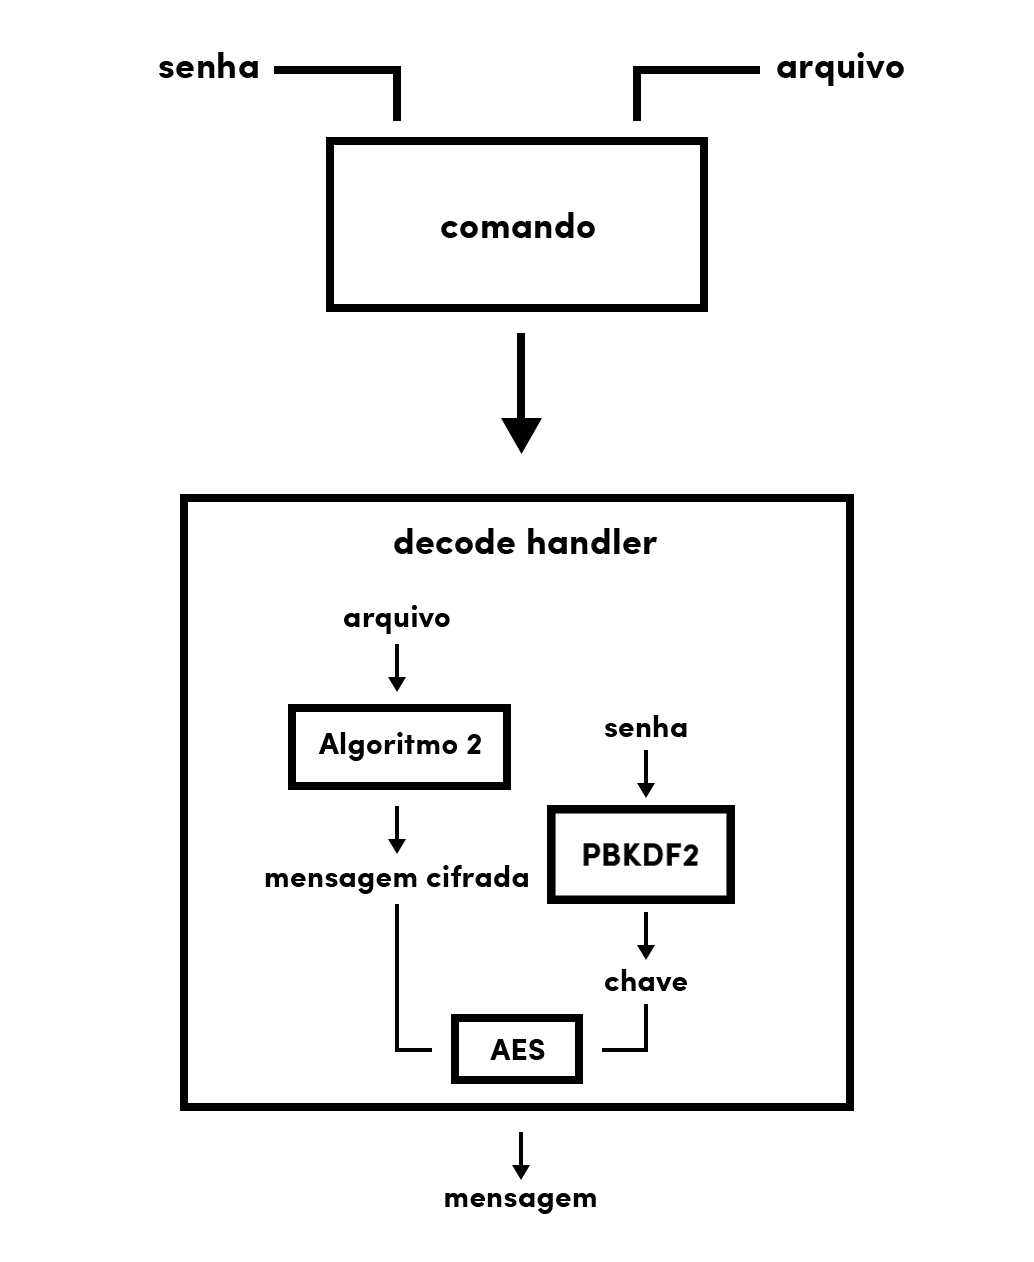
\includegraphics[width=10cm]{images/TCC5.png}
     \legend{Autor: Imagem produzida pelo Autor}
     \label{fig:decode}
\end{figure}

\subsection{Execução e Utilização da Aplicação}

Todo o código desenvolvido está disponível de forma pública no repositório \textit{git} localizado em \href{https://github.com/leviosar/tcc}{https://github.com/leviosar/tcc}, para instalar e executar é necessário possuir uma instalação da linguagem \textit{Python} em sua versão 3.11 ou superior e o gerenciador de pacotes \textit{Poetry}. Após clonar o repositório basta seguir as instruções contidas no arquivo \texttt{README.md} localizado no diretório \textit{src} do projeto.

Como mencionado anteriormente a aplicação implementada utiliza uma interface de linha de comando para responder à entrada do usuário, seguindo os padrões estabelecidos pela especificação POSIX para interpretação de opções, argumentos e caminhos de sistema, no trecho de código abaixo está descrita a utilização do programa a partir de sua interface 

\vspace{10mm}

\begin{lstlisting}[language=bash]
> python -m steganossaurus --help

Usage: python -m steganossaurus [OPTIONS] COMMAND [ARGS]...

Options:
  --help  Show this message and exit.

Commands:
  decode   Recover a message from the given FILE, decrypting it with a required password.
  encode   Embeds a message into the given FILE, encrypting it with a required password.
\end{lstlisting}

\vspace{10mm}

Primeiramente pode ser utilizado o argumento \texttt{\-\-help} sem nenhum comando para retornar mais informações sobre o programa, resultando em um curto guia de uso dos argumentos e disponibilização da lista de comandos.

\vspace{10mm}

\begin{lstlisting}[language=bash]
> python -m steganossaurus encode --help

Usage: python -m steganossaurus encode [OPTIONS] FILE MESSAGE

  Embeds a message into the given FILE, encrypting it with a required password.

Options:
  -o, --output PATH          Path to output file, created if not exists.
  --log-level                Level of data to de logged.
  --password                 Password used to encrypt the message.
  --help                     Show this message and exit.

> python -m steganossaurus encode ./input "steganographia" -o ./output

Password: **********
Repeat for confirmation: **********
Message was encoded at ./output
\end{lstlisting}

\vspace{10mm}

Em seguida o usuário pode chamar do comando \texttt{encode} com o argumento \texttt{\-\-help} que retorna instruções específicas para utilização do comando, como as opções disponíveis, a ordem e o nome dos argumentos. O comando \texttt{encode} então é invocado utilizando como argumentos um arquivo de entrada, uma mensagem para ser codificada pelo algoritmo e como opção um arquivo de saída. A aplicação então requer a digitação e confirmação de uma senha para o a mensagem criptografada e processa a solicitação do usuário, inserindo a mensagem no arquivo utilizando o Algoritmo \ref{alg:one} e gerando um estego-objeto no caminho fornecido.

\vspace{10mm}

\begin{lstlisting}[language=bash]
> python -m steganossaurus decode --help

Usage: python -m steganossaurus decode [OPTIONS] FILE

  Recover a message from the given FILE, decrypting it with a required password.

Options:
  --log-level               Level of data to de logged.
  --password TEXT           Password used to encrypt the message.
  --help                    Show this message and exit.

> python -m steganossaurus decode .\output

Password: **********
Repeat for confirmation: **********
Message found: steganographia
\end{lstlisting}

\vspace{10mm}

Para o processo de decodificação também é oferecida a opção de consultar a documentação do comando a partir da opção \texttt{\-\-help} que retorna todas as informações necessárias para a utilização do comando \texttt{decode}. Para finalizar o ciclo de vida da aplicação o usuário invoca o comando de decodificação passando como argumento o estego-objeto gerado no passo anterior, a aplicação solicita a senha e caso confirmada extrai a mensagem utilizando o Algoritmo \ref{alg:two}, descriptografa com a chave gerada a partir da senha informada e retorna a mensagem em texto plano para o usuário.


